\section{Obvody pro předzpracování signálu}
-důvody použití, využití multiplexeru a demultiplexeru, invertované a neinvertované sítě, diferenční sítě - příklady zapojení funkce.

\subsection{Důvody použití}
Multiplexery a demultiplexery se používají z důvodu nutnosti snímat více vstupů (ADC) nebo budit více výstupů (DAC). Zesílení se poté používá pro zesílení vstupní veličiny, což snižuje náchylnost na šum a usnadňuje jeho převod z analogového do digitálního signálu.

\subsection{Zesilovače s elektronicky přepínaným zesílením}
Elektronické přepínání zesílení lze realizovat pomocí relé, což však má značné nevýhody jako je krátká životnost, doba potřebná k sepnutí je dlouhá, nehodí se pro IO kvůli větším rozměrům, nutnost doplnit budicí obvody pro ovládání úrovněmi TTL => elektronické spínače resp. integrované analogové řadiče (multiplexory a demultiplexory - AMUX)
\subsubsection{Zesilovače pro méně náročné aplikace}
AMUX nahrazuje mechanický spínač, čímž se uplatňuje odpor zapnutého kanálu v řádech desítek až stovek $\Omega$.
\begin{figure}[h]
   \begin{center}
     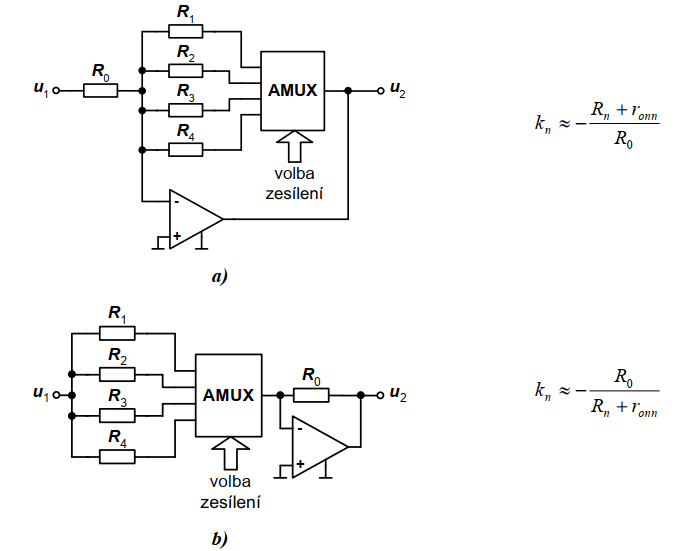
\includegraphics[scale=0.6]{images/Amux1.png}
   \end{center}
   \caption{Přímé přepínání zpětnovazební sítě pomocí AMUX}
\end{figure}

Zesílení lze adjustovat změnou R\textsubscript{n}, tím se ale neodstraní nelineární změny r\textsubscript{on} v závislosti na teplotě a protékajícím proudu. V případě zapojení na a) může dojít k parazitní modulaci r\textsubscript{on}, což ve druhém případě nenastane, protože je AMUX připojen k virtuální nule OZ. Je však citlivější na rušení.

Nenulový odpor spínače r\textsubscript{on} se potlačí zařazením AMUX mimo zpětnovazební síť jak je ukázáno na \ref{fig:AMUX2}.
\begin{figure}[h]
   \begin{center}
     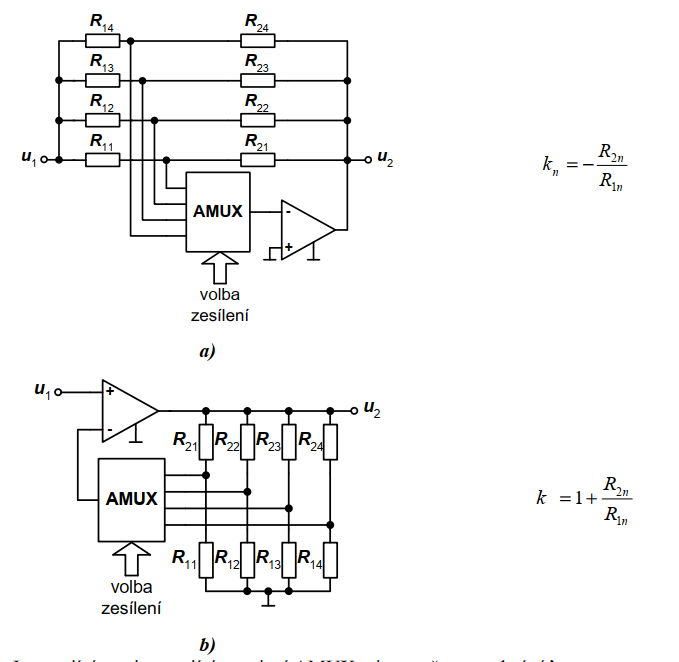
\includegraphics[scale=0.6]{images/Amux2.png}
   \end{center}
   \caption{Invertující a neinvertující zapojení AMUX mimo zpětnovazební síť}
   \label{fig:AMUX2}
\end{figure}

\begin{figure}[h]
   \begin{center}
     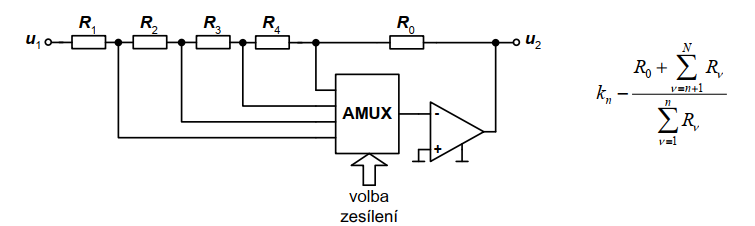
\includegraphics[scale=0.6]{images/Amux3.png}
   \end{center}
   \caption{Jiný způsob invertujícího zapojení s AMUX}
\end{figure}

\begin{figure}[h]
   \begin{center}
     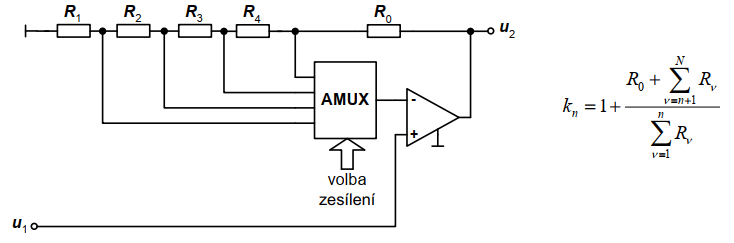
\includegraphics[scale=0.6]{images/Amux4.png}
   \end{center}
   \caption{Upravené neinvertující zapojení}
\end{figure}

Při velkých vstupních signálech se předřazuje dělič, což má výhodu v tom, že se nepřepíná zpětnovazební síť OZ, a proto se při přepínání nemění kmitočtová charakteristika:
\begin{figure}[h]
   \begin{center}
     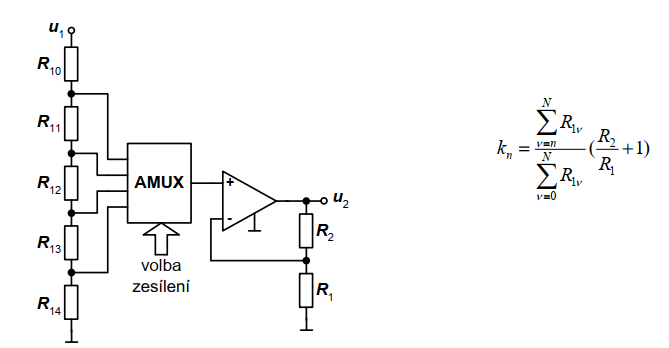
\includegraphics[scale=0.6]{images/Amux5.png}
   \end{center}
   \caption{Využití předřazeného děliče pro velké vstupní signály}
\end{figure}

Snahy zlepšit vlastnosti vedly k přesunutí AMUX až do vnitřní struktury OZ – programovatelný zesilovač. Vstupní odpor však již není tak velký jako u neinvertujícího zesilovače, protože diferenční zesilovače, které jsou právě vyřazeny z činnosti, nejsou provozovány v režimu bootstrap.

Předřazení AMUX před invertující vstup OZ sice potlačilo vliv spínacího odporu, ale zhoršuje šumové poměry – přívody od zpětnovazební sítě přes AMUX až k invertujícímu vstupu OZ jsou kritické (působí jako přijímací anténa), multiplexor sám je také zdrojem šumu (zapnutý kanál generuje praskavý šum, nízkofrekvenční šum, tepelný šum apod.).
\begin{figure}[h]
   \begin{center}
     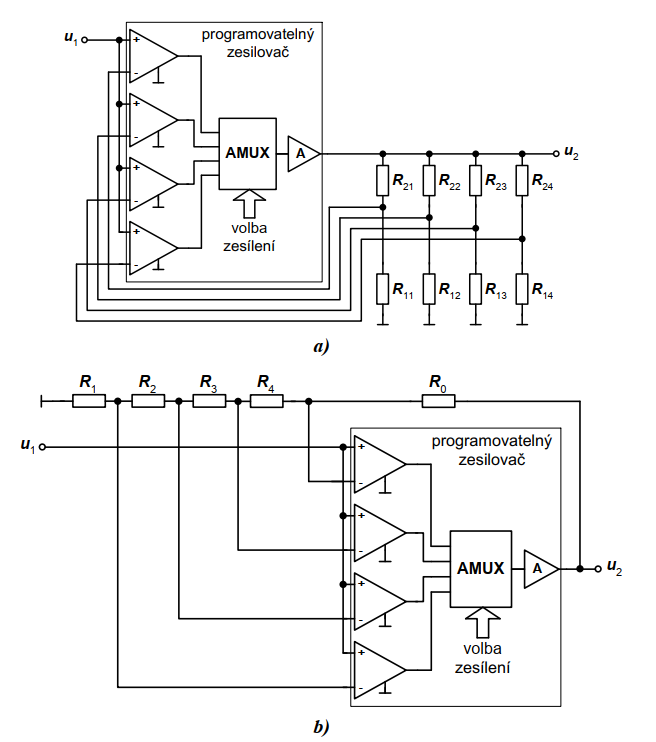
\includegraphics[scale=0.6]{images/Amux6.png}
   \end{center}
   \caption{Doporučované způsoby připojení zpětnovazební sítě k programovatelnému zesilovači}
\end{figure}

\pagebreak
\subsubsection{Přesný analogový demultiplexor}
Je to základní stavební jednotka zesilovačů s elektronicky přepínaným zesílením. Myšlenkou je zařazení AMUX do přímé větve zpětnovazební smyčky, ale až za OZ.

Pro invertující zapojení platí:
\begin{equation}
u_{2n}=-\frac{R_{2n}}{R_{1}}*u_{1}
\end{equation}

Pro neinvertující zapojení platí:
\begin{equation}
u_{2n}=(1+\frac{R_{2n}}{R_{1}})*u_{1}
\end{equation}

\begin{figure}[h]
   \begin{center}
     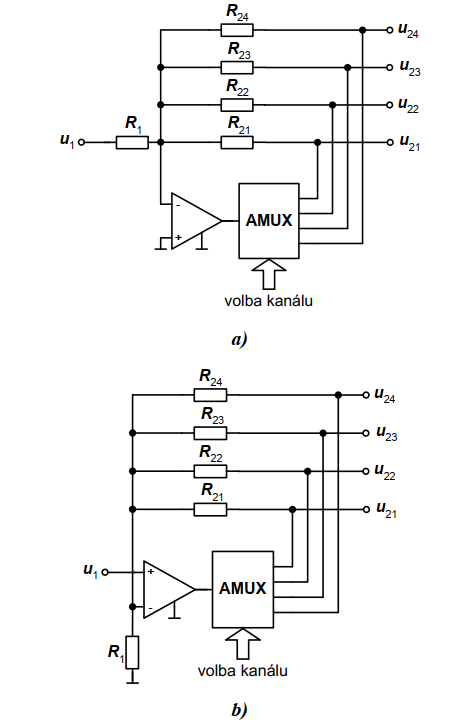
\includegraphics[scale=0.6]{images/Amux7.png}
   \end{center}
   \caption{Invertující a neinvertující zapojení AMUX za OZ}
\end{figure}

\subsection{Analogové multiplexery}
Používají se pro přepínání signálových cest. Obvykle se požaduje, aby bylo možno v každé cestě nastavit popř. dostavit zesílení. Zapojení opět vycházejí z předchozích schémat. Na Obr. \ref{fig:AMUX8}a) a b) jsou uvedena zapojení pro invertující a neinvertující variantu. Diferenční zapojení a schéma s programovatelným zesilovačem jsou analogická.
\begin{figure}[h]
   \begin{center}
     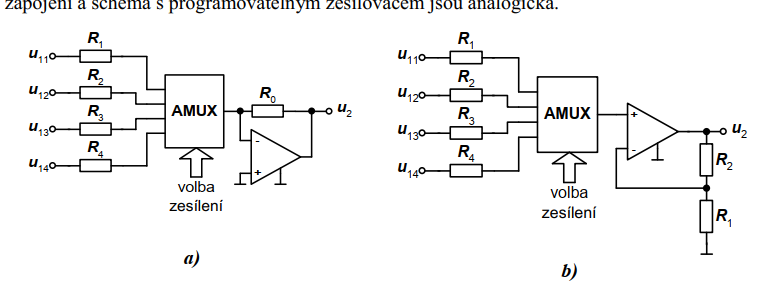
\includegraphics[scale=0.5]{images/Amux8.png}
   \end{center}
   \caption{Invertující a neinvertující zapojení multiplexeru}
   \label{fig:AMUX8}
\end{figure}

Pro zapojení na Obr. \ref{fig:AMUX8}a) platí:
\begin{equation}
u_{2}=-u_{1n}*\frac{R_{0}}{R_{n}+r_{onm}}
\end{equation}

Pro zapojení na Obr. \ref{fig:AMUX8}b) platí:
\begin{equation}
u_{2}=(1+\frac{R_{0}}{R_{n}})*u_{1n}
\end{equation}



























